%!TEX encoding = IsoLatin

%% Document is article 
\documentclass[a4paper]{report}

%% ----------------------------------------------------- PACKAGES ----------------------------------------------------- %%
\usepackage{coolReport}
\usepackage{algorithm2e}
\graphicspath{{./Images/}}
\cRTitle{Semester project report}

%% ---------------------------------------------------------TITLE --------------------------------------------------------- %%

%% ---------------------------------------------------- DOCUMENT ---------------------------------------------------- %%
\begin{document}
	%!TEX encoding = IsoLatin


%% ------------------------------------------------------- PATHS ------------------------------------------------------- %%

%% --------------------------------------------------- PAGE STYLE --------------------------------------------------- %%

%% ---------------------------------------------------- DOCUMENT ---------------------------------------------------- %%


\begin{titlepage}
        	{\sffamily
	\large
        		\noindent \'ECOLE POLYTECHNIQUE FEDERALE DE LAUSANNE \\
        		MT SECTION\\
        		FAURY Louis \\
        	}
	
	\vfill 
        \begin{center}
   		{\sffamily\Huge
         		\textbf{SEMESTER PROJECT REPORT} \\
			\vspace{0.3cm}
			\Large
			\textbf{LASA}
		}
		\vspace{1cm}
	
        		
\includegraphics[width=0.8\textwidth]{epfl_logo.png}
        
        		\vspace{1cm}
         
         	\sffamily\huge\textbf{ 	
\titlebox{0.95}{\sffamily\huge\textbf{Learning from suboptimal demonstrations: the role of compliance in the exploration-exploitation trade-off}} }
        \end{center}
        
	\vspace{2cm}
         \centering
\includegraphics[width=0.1\textwidth]{sepLine}
         \vspace{0.2cm}

	\large
        \begin{center}
		\begin{tabular}{rl}
    			\textbf{Laboratory} & Learning Algorithms and Systems Laboratory (LASA)\\
			\textbf{Professor} & Prof. Aude Billard \\
    			\textbf{Supervisors} & Mahdi Khoramshahi and Andrew Sutcliffe\\
			\textbf{Semester} & Spring 2017\\
		\end{tabular}
	\end{center}
	\vspace{0.05cm}
         \centering
\includegraphics[width=0.1\textwidth]{sepLine}
         \vspace{0.6cm}
         \vfill
\end{titlepage}

	
	\tableofcontents
	
	\chapter{Introduction}
	{
		\section{Motivations}
		{
			
		}
		\section{Background}
		{
			\subsection{Learning from demonstration}
			{
			
			}
			\subsection{Transfer learning}
			{
			
			}
		}
		\section{Proposed approach}
		{

		}
	}
	\newpage
	
	\chapter{Reinforcement Learning}
	{
		\section{Formulation}
		{
			\subsection{Notations and first definitions}
			{
				\paragraph{} Reinforcement learning is a framework in which an \emph{agent} (or a \emph{learner}) learns its actions from interaction with its environment. The environment generates scalar values called \emph{rewards}, that the agent is seeking to maximize over time. 
			
				\paragraph{} Let $\mathcal{S}$ denote the state space in which our agent evolves (the localization of a robot on a grid for instance), and $\forall{s}\in\mathcal{S}$ we will define the action state $\mathcal{A}(s)$, describing all possible action that can be taken by the agent at state $s$. When taking an action from a state $s_t$, the agent finds itself in a new state $s_{t+1}$ where it receives a reward $r_{t+1}\in\mathbb{R}$. The action taken is sampled over a probability distribution from the joint space of state and action : 
				\begin{equation}
					\begin{aligned}
						\pi \, : \, \mathcal{S}\times\mathcal{A}(s) \, &\to [0,1]\\
							 (s,a) \, &\to \,  \pi(s,a)
					\end{aligned}
				\end{equation}	
				where $\pi(s,a)$ is the probability of picking action $a$ in state $s$. Such a distribution is called the agent's \emph{policy}. The key goal of reinforcement learning is teaching an agent on how to change its policy to maximize its reward on the long run. 
				
				\paragraph{} The agent indeed seeks to maximize the \emph{expected return} $R_t$ mapping the reward sequence into $\mathbb{R}$. A commonly used expression for this value employs a \emph{discount factor} $\gamma \in [0,1]$, allowing to make the agent's more sensible to rewards it will get in a close future : 
				\begin{equation}
					R_t = \sum_{i=0}^T \gamma^i r_{t+1+i}
				\end{equation}
				This also allows to adapt this formulation to continuous tasks, where there are no terminal states and the task goes on indefinitely (there are no \emph{episodes} in the learning). 
				
				%% TODO : quote Sutton's book 
			}
			\subsection{Markov decision process}
			{
				\paragraph{} To make the problem tractable, we ask for the state signal to comply with Markov's property, hence to be \emph{memory-less}. For instance, we want to be able to write that, in a stochastic environment, $\forall s'\in\mathcal{S}$ : 
				\begin{equation}
					\mathbb{P}\left( s_{t+1}=s' \, \vert \, a_t, s_t, \hdots, a_1,s_1\right) = \mathbb{P}\left( s_{t+1}=s' \, \vert \, s_t, a_t\right)
				\end{equation}
				
				\paragraph{} Hence, every reinforcement learning problem can be represented by a \emph{Markov Decision Process}, that consists in a 5-tuple $\left(\mathcal{S}, \mathcal{A}, \mathcal{P}_{\cdot}(\cdot,\cdot), \mathcal{R}_{\cdot}(\cdot), \gamma \right)$ where : 
				\begin{itemize}[label=$\triangleright$]
					\item $\mathcal{S}$ is the agent's state space
					\item $\mathcal{A}$ is the agent's action space
					\item $\forall s,s'\in\mathcal{S}, \, \forall a\in\mathcal{A}(s)$,  $\mathcal{P}_a(s,s') = \mathbb{P}(s_{t+1}=s'\, \vert \, s_t = s, a_t = a)$ is the probability that action $a$ in state $s$ will lead the agent to transitioning to state $s'$.
					\item $\forall s,s'\in\mathcal{S}, \, \forall a\in\mathcal{A}(s)$,  $\mathcal{R}_a(s,s')$ is the immediate reward perceived by the agent when transitioning from state $s$ to $s'$ when taking action $a$. 
					\item $\gamma$ is the discount factor. 
				\end{itemize}
				
				\paragraph{} A \emph{finite Markov decision process} designates a MDP for which both the action and state space are finite. 
			}
			\subsection{State and action value function}
			{
				\paragraph{} Most of the reinforcement learning algorithms are based on evaluation value function. A value function is a function mapping the state space in $\mathbb{R}$, estimating how good (in terms of expected future reward) it is for the agent to be in a given space. More precisely, a value function $V^\pi(\cdot)$ evaluates the expected return of a state when following the policy $\pi$. $V^\pi(\cdot)$ is called the \textbf{state-value function}. 
				\begin{equation}
					\forall{s}\in\mathcal{S}, \quad V^\pi(s) = \E[\pi]{R_t \, \vert \, s_t = s}
				\end{equation}
				The \textbf{action-value function} evaluates the value of taking a given action, and then following the policy $\pi$ : 
				\begin{equation}
					\forall{s,a}\in\mathcal{S}\times\mathcal{A}(s), \quad Q^\pi(s,a) = \E[\pi]{ R_t \, \vert \, s_t=s, \, a_t=a}
				\end{equation}
				
				\paragraph{} Both those functions satisfy particular recursive relationships known as the \emph{Bellman equations}. It is shown that (see TODO quote Sutton) we have the following results : 
				\vspace{10pt}
				
				\coolbox{white}{\textcolor{black}{Bellman equations for Markov Decision Process}}
				{
					\begin{itemize}[label=$\triangleright$]
						\item Bellman equation for the state-value function : $\forall s \in\mathcal{S}$ 
						\begin{equation}
							V^\pi(s) = \sum_{a\in\mathcal{A}}\pi(s,a)\sum_{s'} \mathcal{P}_a(s,s')\left[\mathcal{R}_a(s,s') + \gamma V^\pi(s')\right]
						\end{equation}
						\item Bellman equation for the action value function : $\forall{s,a}\in\mathcal{S}\times\mathcal{A}(s)$ : 
						\begin{equation}
							Q^\pi(s,a) = \sum_{s'}\mathcal{P}_a(s,s')\left[ \mathcal{R}_a(s,s') + \gamma V^\pi(s')\right]
						\end{equation}
					\end{itemize}
				}
			}
			\subsection{Optimal policies}
			{
				\paragraph{} The value functions define a partial ordering in the policy space. A policy $\pi$ is therefore said to be better than $\pi'$ (or $\pi\geq \pi'$) if $\forall{s}\in\mathcal{S}$, $V^\pi(s) \geq V^\pi(s')$. We are looking for $\pi^*$ so that : 
				\begin{equation}
					\forall\pi, \quad \pi^* \geq \pi 
				\end{equation}
				
				TODO quote showed that for finite MDPs, there is always at least one policy that is better our equal to all others, and therefore is called the \emph{optimal policy} $\pi^*$. As shown in TODO quote, the state-value and action-value function verify the \emph{Bellman optimality equations}. 
				
				\vspace{10pt}
				
								\coolbox{white}{\textcolor{black}{Bellman optimality equations}}
				{
					\begin{itemize}[label=$\triangleright$]
						\item Bellman optimality equation for the state-value function : $\forall s \in\mathcal{S}$ 
						\begin{equation}
							V^\pi(s) = \max_{a\in\mathcal{A}(s)}\pi(s,a)\sum_{s'} \mathcal{P}_a(s,s')\left[\mathcal{R}_a(s,s') + \gamma V^\pi(s')\right]
						\end{equation}
						\item Bellman optimality equation for the action value function : $\forall{s,a}\in\mathcal{S}\times\mathcal{A}(s)$ : 
						\begin{equation}
							Q^\pi(s,a) = \sum_{s'}\mathcal{P}_a(s,s')\left[ \mathcal{R}_a(s,s') + \max_{a\in\mathcal{A}(s')} Q(s',a') \right]
						\end{equation}
					\end{itemize}
				}
				
				\paragraph{} Those relations are essential in understanding the solving algorithms that will be presented later. 
			}
		}


			\paragraph{} There exists several ways of solving (i.e computing the optimal policy) of a Markov Decision Process, that can generically be separated in two categories : \emph{model-based} and \emph{model-free} methods. 
		\section{Dynamic Programing}
		{
			\paragraph{} Dynamic programing is a mathematically well-developed theory. It requires the complete and accurate model of the environment, making it a model-based method. 
			
			\paragraph{} Dynamic programing methods aims at computing the optimal value function at every state of state space. This could, of course, be done by solving the $\vert \mathcal{S} \vert $ equations of $\vert \mathcal{S} \vert $ unknowns that are the Bellman equations for a given policy, and then evolve that policy toward a better one, based on the current value function. Of course, this approach is computationally intractable for large state space and therefore needs to be adapted, but gives a first approach of the idea behind dynamic programing. 
				
			\subsection{Generalized policy iteration}
			{
				\paragraph{} The generalized policy iteration methods rely on alternating two processes, known as \textcolor{red}{policy evaluation} and \textcolor{red}{policy improvement}. 
				\begin{itemize}[label=$\triangleright$]
					\item Policy evaluation deals with estimating the value function of a given policy $\pi$, without directly solving the full system given by Bellman equations. The idea is actually pretty simple : use Bellman's equation as an update rule, using that the value function is a fixed point for this update rule. The algorithm, after setting the tabled value function to an initial value, iterate by performing what is called \emph{full Bellman backups} : 
					\begin{equation}
						\forall{s}\in\mathcal{S}, \quad V_{k+1}^\pi(s) = \sum_{a\in\mathcal{S}} \pi(s,a)\sum_{s'}\mathcal{P}_a(s,s') \left[\mathcal{R}_a(s,s')+V_k^\pi(s')\right]
					\end{equation}
					This algorithm converges under the same assumptions that guarantee the existence of the value function, and has the generic name of \emph{iterative policy evaluation}. They are many refining for speeding up that process (reduced backups, prioritized sweeping) that we won't address here. 
				\item Policy evaluation is a process that from a given policy value function, returns a better or equal policy compared to the latter. The simplest way to do that is for every state $s\in\mathcal{S}$, consider every action-value functions : 
				\begin{equation}
					Q(s,a) = \sum_{s'}\mathcal{P}_a(s,s')\left[\mathcal{R}_a(s,s') + \gamma V\pi(s')\right], \quad a\in\mathcal{A}(s)
				\end{equation}
				and to build $\pi'$ to be \emph{greedy} with respect to those actions-values : 
				\begin{equation}
					\pi'(s) = \argmax{a\in\mathcal{A}(s)}{Q(s,a)}
				\end{equation}
					The policy improvement theorems then ensures that $\pi'\geq \pi$. 
				\end{itemize}
				
				\paragraph{} Hence, generalized policy improvement are a set of methods that iteratively combine those two sub-methods to compute the optimal policy for a given MDP. Of course, one does not have to perform all sweeps of value evaluation before improving the policy to converge toward an optima (indeed, many times our sweeps won't have any affect on the greedy policy). They are many ways to combine the two (prioritized sweeping, asynchronous dynamic programing), but the most used and one of the most quickest way to converge is to use the value iteration algorithm. 
			}	
			\subsection{The value iteration algorithm}
			{
				\paragraph{} The value iteration algorithm takes the limit of the behavior we just described, and stops the value evaluation procedure after only \emph{one state space sweep}. It therefore performs a simple backup procedure : 
					\begin{equation}
						\forall{s}\in\mathcal{S}, \quad V_{k+1}  = \max_{a\in\mathcal{A}}  \sum_{s'}\mathcal{P}_a(s,s')\left[\mathcal{R}_a(s,s') + \gamma V_k^\pi(s')\right]
					\end{equation}
					For any arbitrary $V_0$, it is shown that $V_k\to V^*$ as $k\to\infty$, under the same hypothesis that ensure the existence of the optimal value function $V^*$. As one can notice, it actually implements the \emph{Bellman optimality conditions} as an update rule !
				}
			}
		
		
		\section{Temporal differences methods}
		{
			\paragraph{} Temporal difference methods can be seen as a combination of dynamic programing and another kind of learning called Monte Carlo methods, where the expected return are approximated via sampling. Like dynamic programming, TD methods are said to bootstrap (meaning that they build their estimators through already estimated values), but are \emph{model-free} methods and learn from experience. 
			
			\paragraph{} The justification, proof of convergences and literature and those models is pretty wide, hence we will not cover them in this report. However, full description of those methods can be found in TODO quote. 
			
			\subsection{On-policy method : SARSA}
			{
				\paragraph{} The SARSA algorithm is an \emph{on-policy} control method, meaning that the algorithm updates the value function and improves the current policy it is following. At state $s_t$, it chooses an action $a_t$ from its policy and follows it. After observing the reward $r_{t+1}$ and the next state $s_{t+1}$, it again chooses an action $a_{t+1}$ using a soft policy and performs a one-step backup : 
				\begin{equation}
					Q(s_t,a_t) \leftarrow Q(s_t,a_t) + \alpha\left[r_{t+1} + \gamma Q(s_{t+1},a_{t+1}) - Q(s_t,a_t)\right]
				\end{equation}
				It therefore relies on a 5-tuple $(s_t,a_t,r_{t+1},s_{t+1},a_{t+1})$ to perform the udpate, giving it the State Action Reward State Action (SARSA) name. 
				\vspace{10pt}
				
				\coolbox{white}{\textcolor{blue}{The General Sarsa Algorithm}}
					{
						\begin{algorithm}[H]
	 					\SetAlgoLined
						\LinesNumbered
						\emph{\textsf{1. Initialize}} $Q(s,a)$ arbitrarily $\forall (s,a)\in\mathcal{S}\times\mathcal{A}(s)$ \\
						\BlankLine
						\BlankLine
						\emph{\textsf{2. Repeat}} for each episode : \\
						\Indp \Indp 
							Initialize $s$ \\
							Choose $a\in\mathcal{A}(s)$ using a soft policy derived from $Q$ (typically $\varepsilon$-greedy) \\
							Repeat for each step of the current episode :   \\
							\Indp \Indp 
								Take $a$, observe $r,s'$ \\
								Choose $a'$ from $s'$ using policy derived from $Q$ 
								$ Q(s,a) \longleftarrow Q(s,a) + \alpha\big[ r + \gamma Q(s',a') - Q(s,a) \big]$ \\
								$a\leftarrow a'$, $s\leftarrow s' $ \\
								
							\Indm \Indm 
						until $s\in\mathcal{S}^+$.
						\Indm \Indm 
						\end{algorithm}
					}
					
					\paragraph{} The convergence properties of SARSA depend on the nature of the policy's dependency on Q. Indeed, SARSA converges with probability 1 to the optimal policy as long as all the sate and actions pairs are visited an infinite number of time, and the policy converges in the limit to the greedy policy. This is done, for instance, by turning the temperate of a softmax based policy to 0, or by having $\eps\to 0$ for a $\eps$-greedy policy. For SARSA to converge, we also as the learning rate to comply with the stochastic approximation conditions : 
					\begin{equation}
						\sum_k \alpha_k(a) = +\infty \quad { and } \quad \sum_k \alpha_k(a)^2 < +\infty
					\end{equation}
					where $\alpha_k(a)$ is the learning rate for the k\textsuperscript{th} visit of the pair $(s,a)$. 
					
			}
			\subsection{Off-policy method : Q-learning}
			{
				\paragraph{} The Q-learning algorithm is an off-policy method who learns to directly approximate $Q^*$, independently of the policy being followed. Its update rule is given by :
				\begin{equation}
					Q(s_t,a_t) \leftarrow Q(s_t,a_t) + \alpha \left[ r_{t+1} + \gamma \max_{a\in\mathcal{A}(s_{t+1})} Q(s_{t+1},a) - Q(s_t,a_t)\right]
				\end{equation}
				The actual policy being followed still has an effect in that it determines which state-actions pairs are visited and updated. However all that is required for convergence it that all pairs continue to be updated. 
				\vspace{10pt}
				
				\coolbox{white}{\textcolor{blue}{Q-Learning Algorithm}}
					{
						\begin{algorithm}[H]
	 					\SetAlgoLined
						\LinesNumbered
						\emph{\textsf{1. Initialize}} $Q(s,a)$ arbitrarily $\forall (s,a)\in\mathcal{S}\times\mathcal{A}(s)$ \\
						\BlankLine
						\BlankLine
						\emph{\textsf{2. Repeat}} for each episode : \\
						\Indp \Indp 
							Initialize $s$ \\
							Repeat for each step of the current episode :   \\
							\Indp \Indp 
								Choose $a\in\mathcal{A}(s)$ using arbitrary policy \\
								Take $a$, observe $r,s'$ \\
								$ Q(s,a) \longleftarrow Q(s,a) + \alpha\big[ r + \gamma \max_{a'\in\mathcal{A}(s')}Q(s',a') - Q(s,a) \big]$ \\
								$s\leftarrow s' $ \\
								
							\Indm \Indm 
						until $s\in\mathcal{S}^+$.
						\Indm \Indm 
						\end{algorithm}
					}
				
				\paragraph{} Along with this hypothesis and a slight variation in the usual stochastic approximation conditions, the learned action value function by Q-learning has been shown to converge to $Q^*$ with probability $1$. 
			}
		}
	
		\section{Grid-world examples}
		{
			\paragraph{} We hereinafter describe two grid-world space, on which we will apply the learning rule derived in the latest section. Such example are trivial and are displayed here just to show convergence and behavior of the different algorithms. 
			
			\paragraph{} We'll consider the two following state space : 
			\begin{figure}[h!]
				\begin{minipage}{0.45\linewidth}
					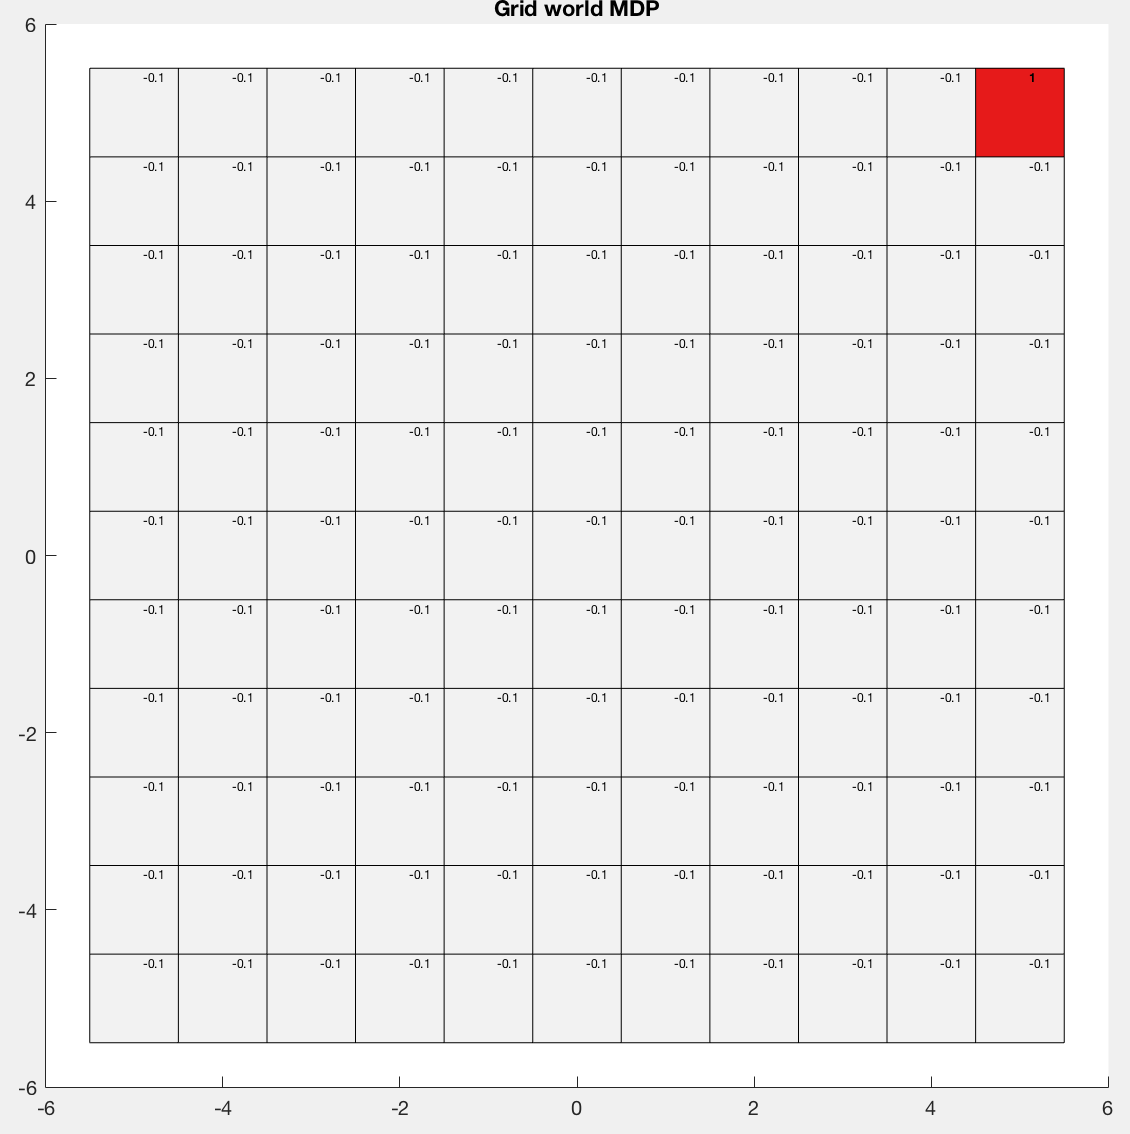
\includegraphics[width=\linewidth]{free_grid}
					\caption{The \emph{free\_grid} state space}
				\end{minipage}
				\hfill
				\begin{minipage}{0.45\linewidth}
					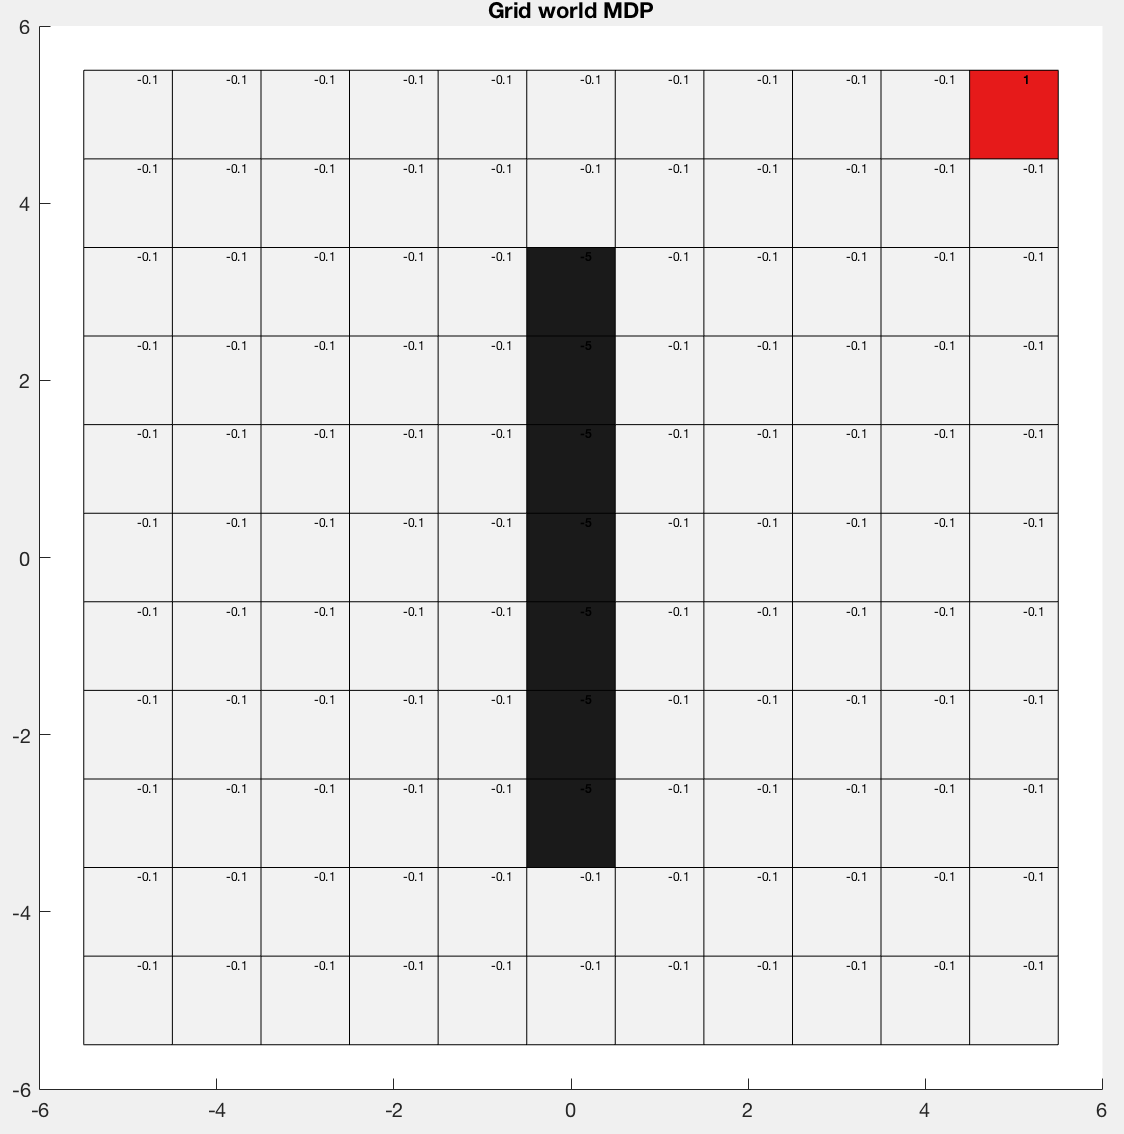
\includegraphics[width=\linewidth]{bar_grid}
					\caption{The \emph{bar\_grid} state space}
				\end{minipage}
			\end{figure}
			\subsection{Dynamic Programing solving}
			{
				\paragraph{} Let us run the DP algorithm on such grid worlds. We'll consider a stochastic environnement, with the transition probability : 
				\begin{equation}
					\mathcal{P}_{s,s'}^a = \left\{\begin{aligned} &0.9 &\text{ if }s' = s(a) \\ &0.1 &\text{ otherwise} \end{aligned}\right.
				\end{equation}
				Running the value iteration algorithm (assuming we now the environment model), we obtain the following policies and learning curves. The stopping criterion adresses the maximum absolute change brought to the value function as the sweeping goes through the state space : 
				\begin{equation}
					\text{ If } \max_{s\in\mathcal{S}} \vert V_{k+1}(s) - V_k \vert < \delta \text{ then stop}
				\end{equation}
				
				\begin{figure}[h!]
				\begin{minipage}{0.45\linewidth}
					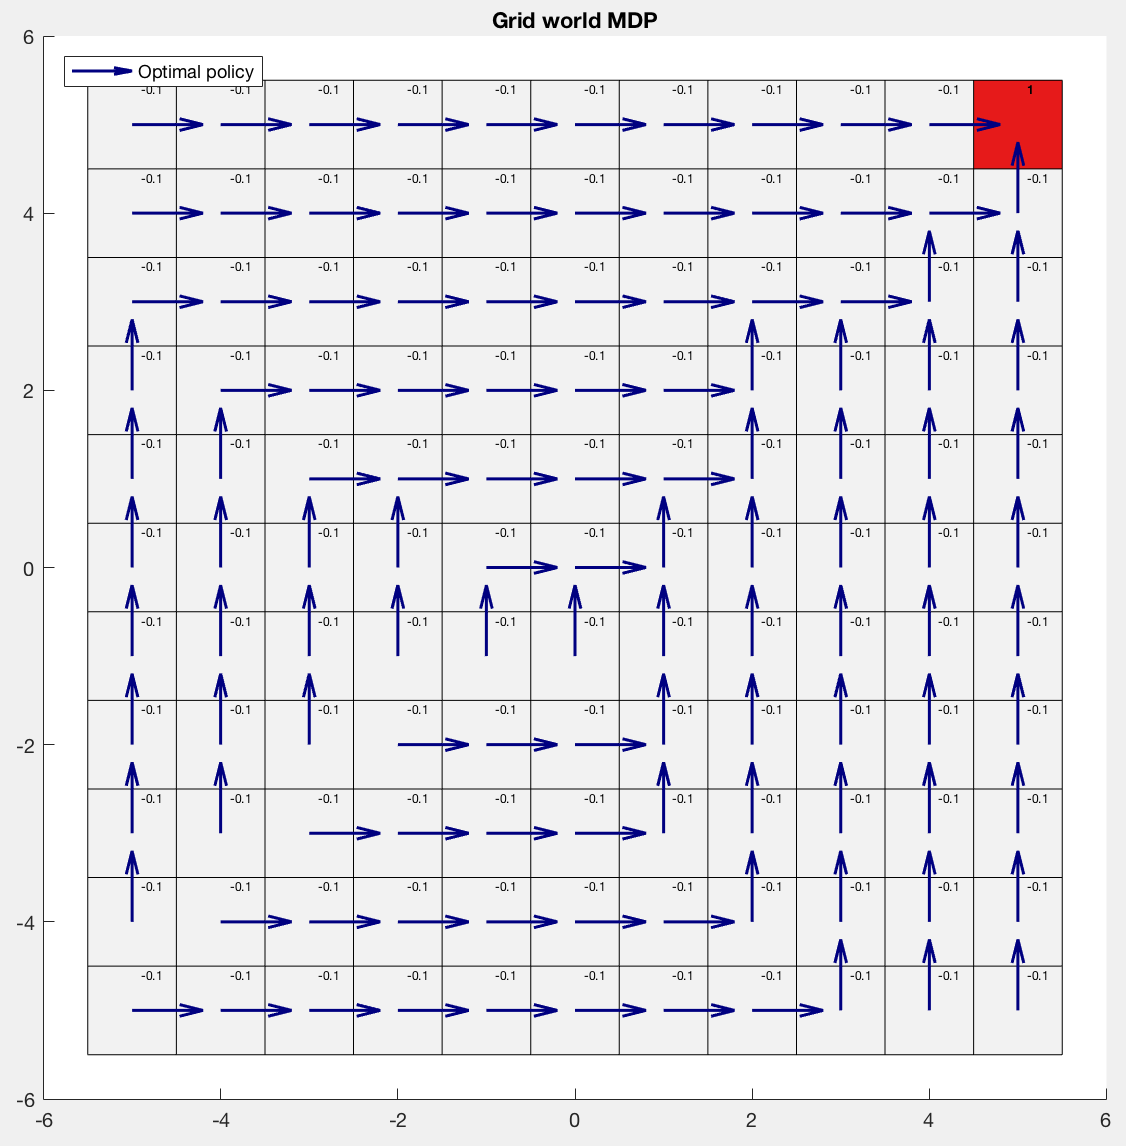
\includegraphics[width=\linewidth]{free_grid_bellman_policy}
					\caption{The \emph{free\_grid} learned optimal policy}
				\end{minipage}
				\hfill
				\begin{minipage}{0.45\linewidth}
					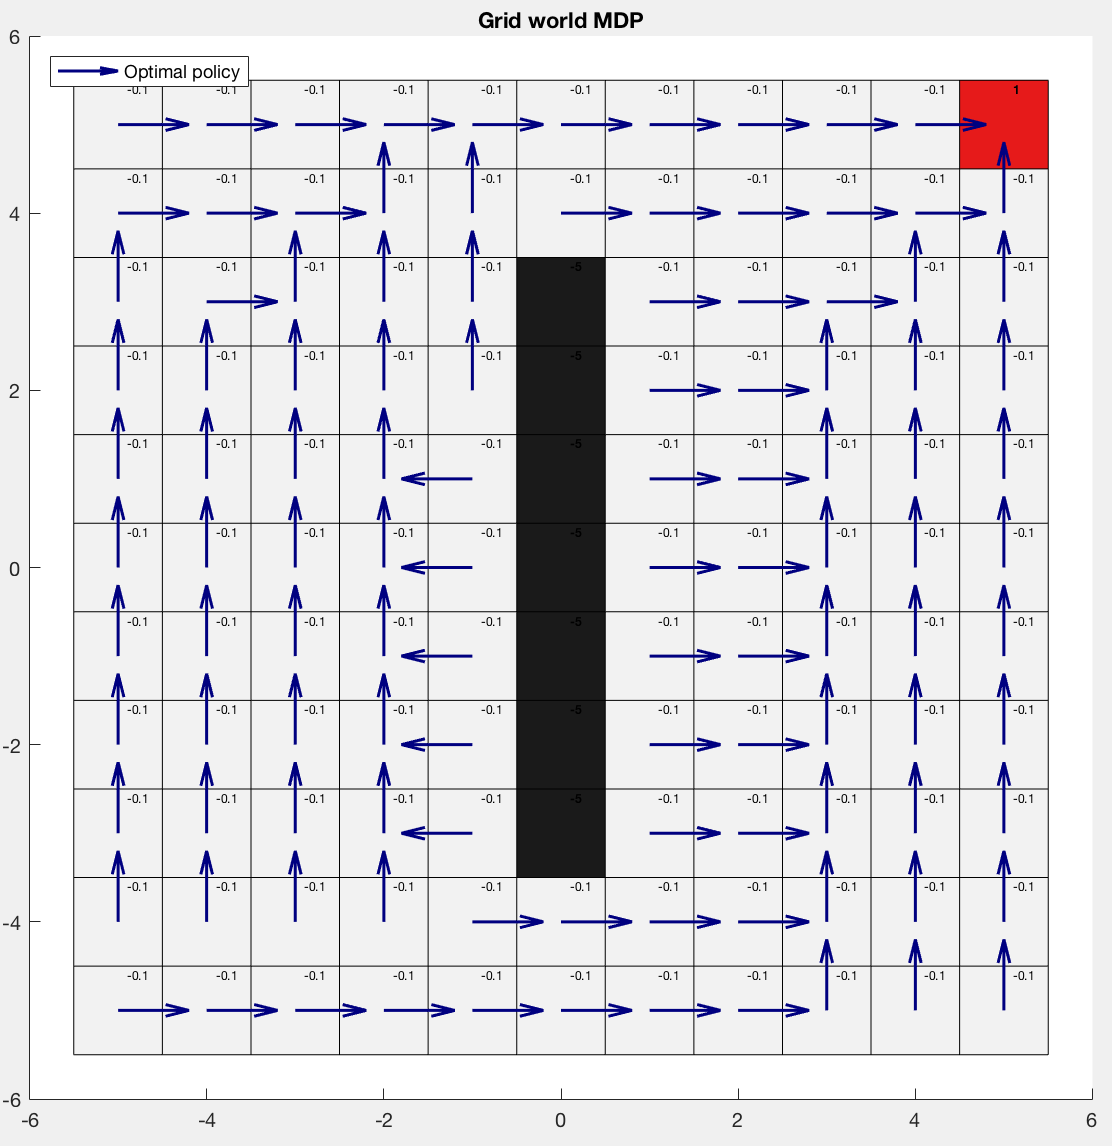
\includegraphics[width=\linewidth]{bar_grid_bellman_policy}
					\caption{The \emph{bar\_grid} learned optimal policy}
				\end{minipage}
				\end{figure}
				
				\begin{figure}[h!]
				\begin{minipage}{0.45\linewidth}
					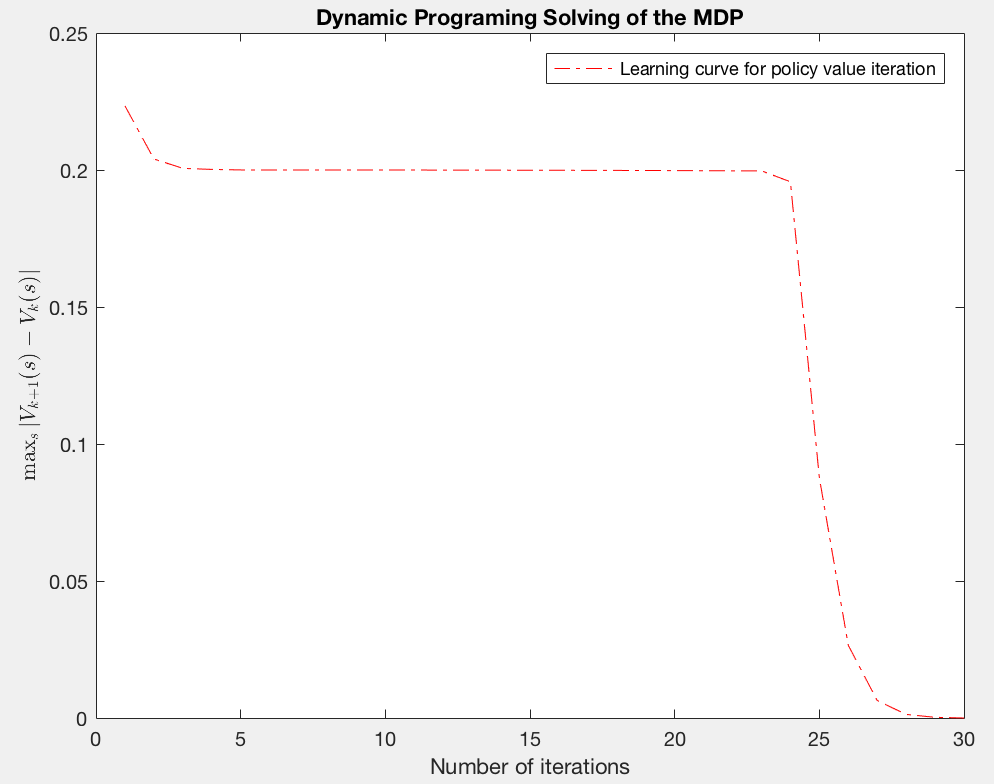
\includegraphics[width=\linewidth]{free_grid_bellman_lc}
					\caption{The \emph{free\_grid} value iteration learning curve}
				\end{minipage}
				\hfill
				\begin{minipage}{0.45\linewidth}
					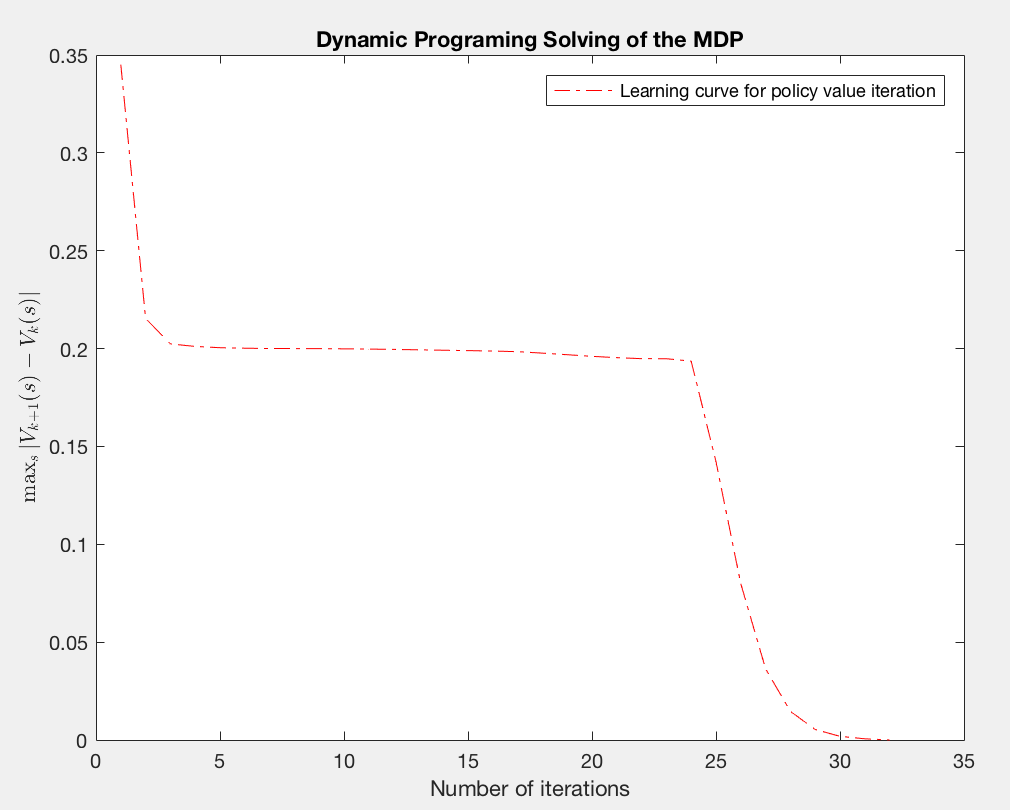
\includegraphics[width=\linewidth]{bar_grid_bellman_lc}
					\caption{The \emph{bar\_grid} value iteration learning curve}
				\end{minipage}
				\end{figure}
				
				\paragraph{} One can notice that for the \emph{bar\_grid} environment, the agent undergoes a longer trajectory than necessary, at the left of the obstacle. This is because of the stochastic nature of the environment, causing the agent to learn to takes its distance with the obstacle in order not to accidentally hit it (and then receive a very negative reward). 
				
				\paragraph{} The learned policy are indeed optimal. The next algorithms (SARSA and Q-learning) will try to reproduce them without a model for the environment. 
			}
			\subsection{SARSA solving}
			{
				\paragraph{} We display here the learning curves for the \emph{free\_grid} state space using SARSA. The algorithm manages to learn the optimal policy and the right action-value functions. We use \emph{optimistic initialization} to encourage exploration, and Gibbs sampling for following a soft-policy : $\forall (s,a) \in\mathcal{S}\times \mathcal{A}(s)$ 
				\begin{equation}
					\pi(s,a) = \displaystyle \frac{ e^{Q(s,a)/\tau}}{\sum_{a'\in\mathcal{A}(s)}e^{Q(s,a')/\tau}}
				\end{equation}
				We'll tune the distribution's temperature $\tau$ to zero, in order to converge toward the greedy policy w.r.t the learned action-value function. 
				
				\paragraph{} Following this strategy and tuning our learning rate to comply with the stochastic approximation conditions, we obtain the following learning curves. Again, our stopping criterion addresses the \emph{maximum change in the acton-value function over all the trajectories of a mini-batch}. 
				\begin{figure}[h!]
					\begin{minipage}{0.4\linewidth}
						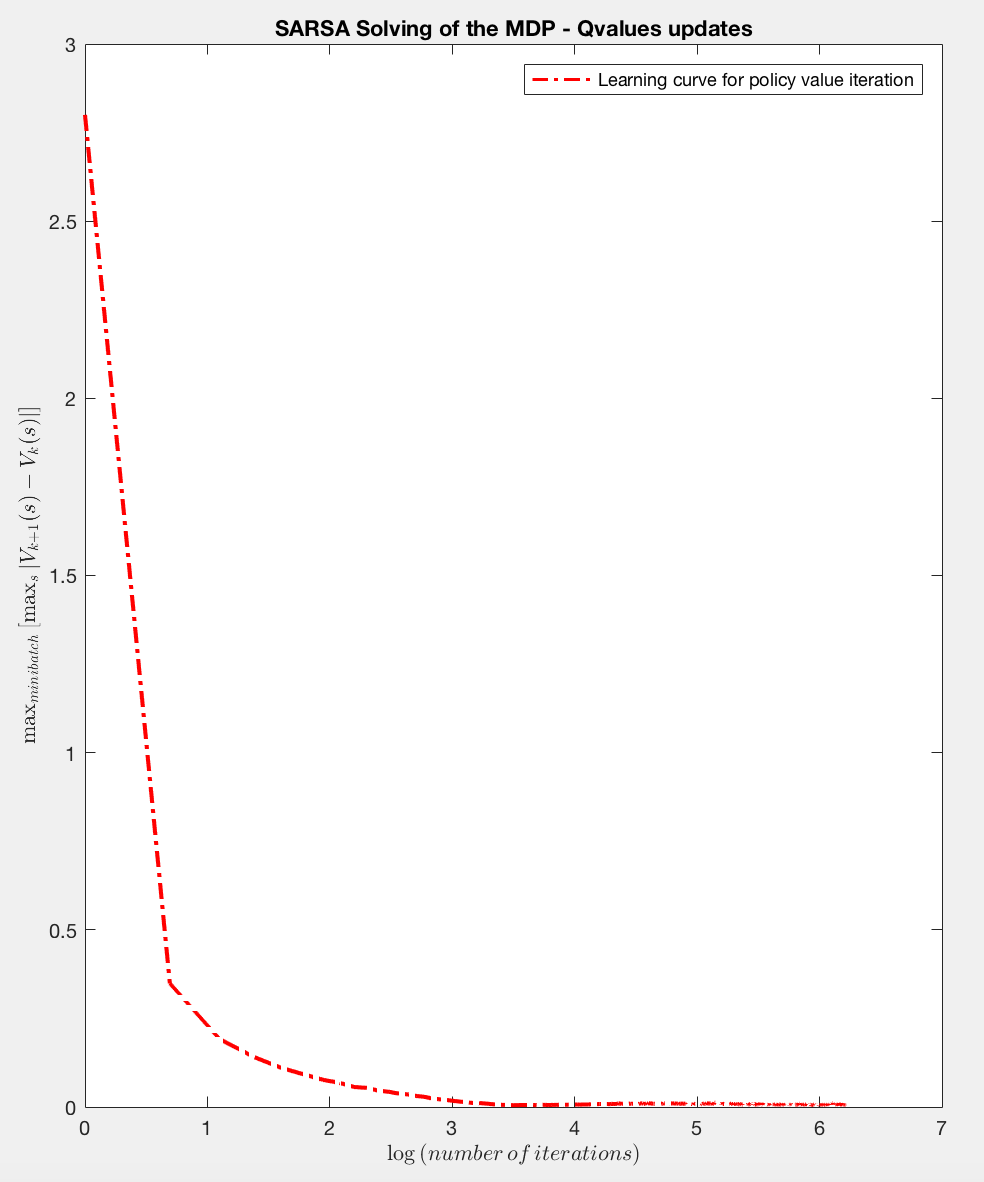
\includegraphics[width=\linewidth]{sarsa_learning_curve_free_grid}
						\caption{Learning curve for SARSA on \emph{free\_grid}}
					\end{minipage}
					\hfill
					\begin{minipage}{0.4\linewidth}
						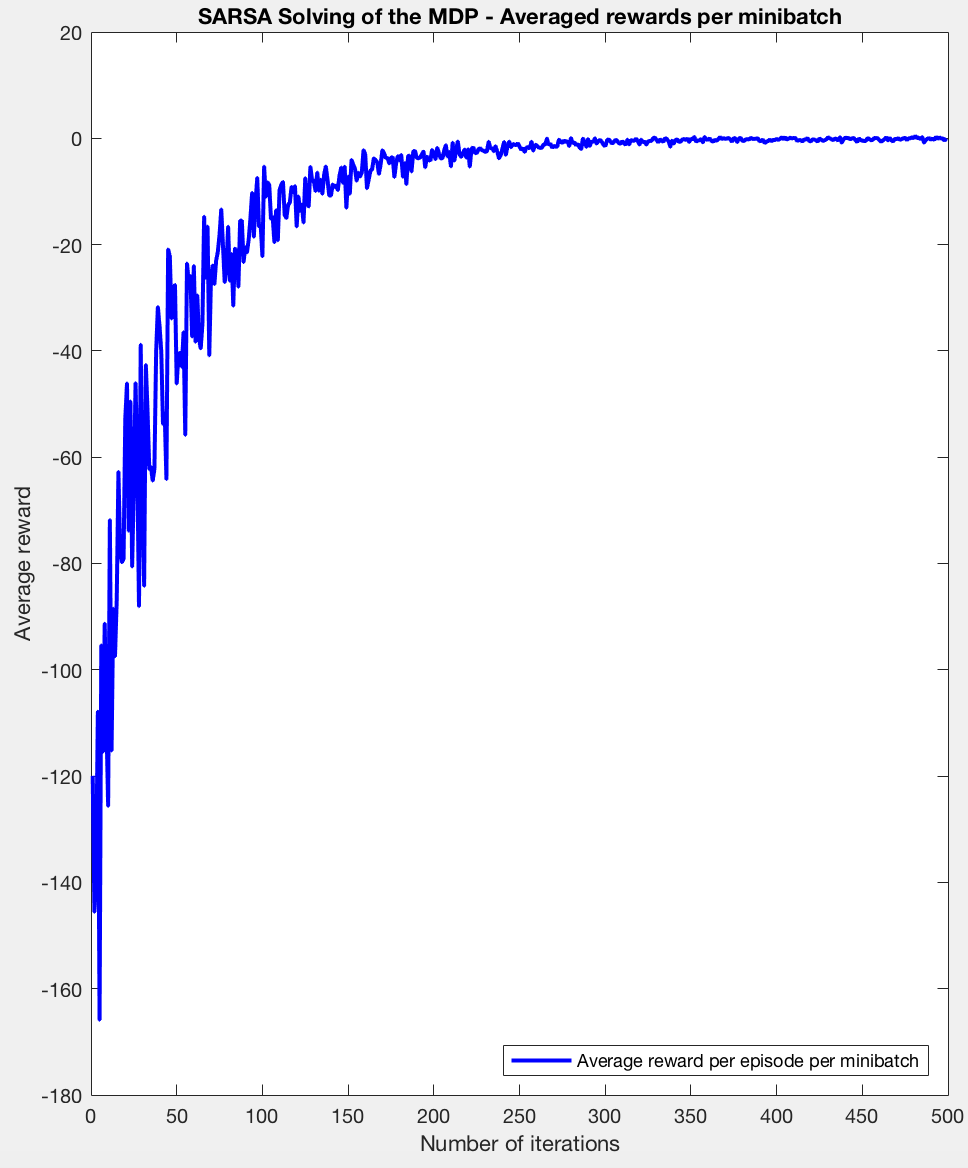
\includegraphics[width=\linewidth]{sarsa_average_rewards_freegrid}
						\caption{Averaged rewards over mini-batch for SARSA on \emph{free\_grid}}
					\end{minipage}
				\end{figure}
				  
			}
			\subsection{Q-learning solving}
			{
				\paragraph{} We display here the learning curves for the \emph{bar\_grid} state space using Q-learning. Again, the algorithm manages to learn the optimal policy and the right action-value functions. We use Gibbs sampling for the behavior policy, without any tuning for the temperature (the behavior policy doesn't need to be greedy in limit). The learning curves obtained are given hereinafter.
				\begin{figure}[h!]
					\begin{minipage}{0.4\linewidth}
						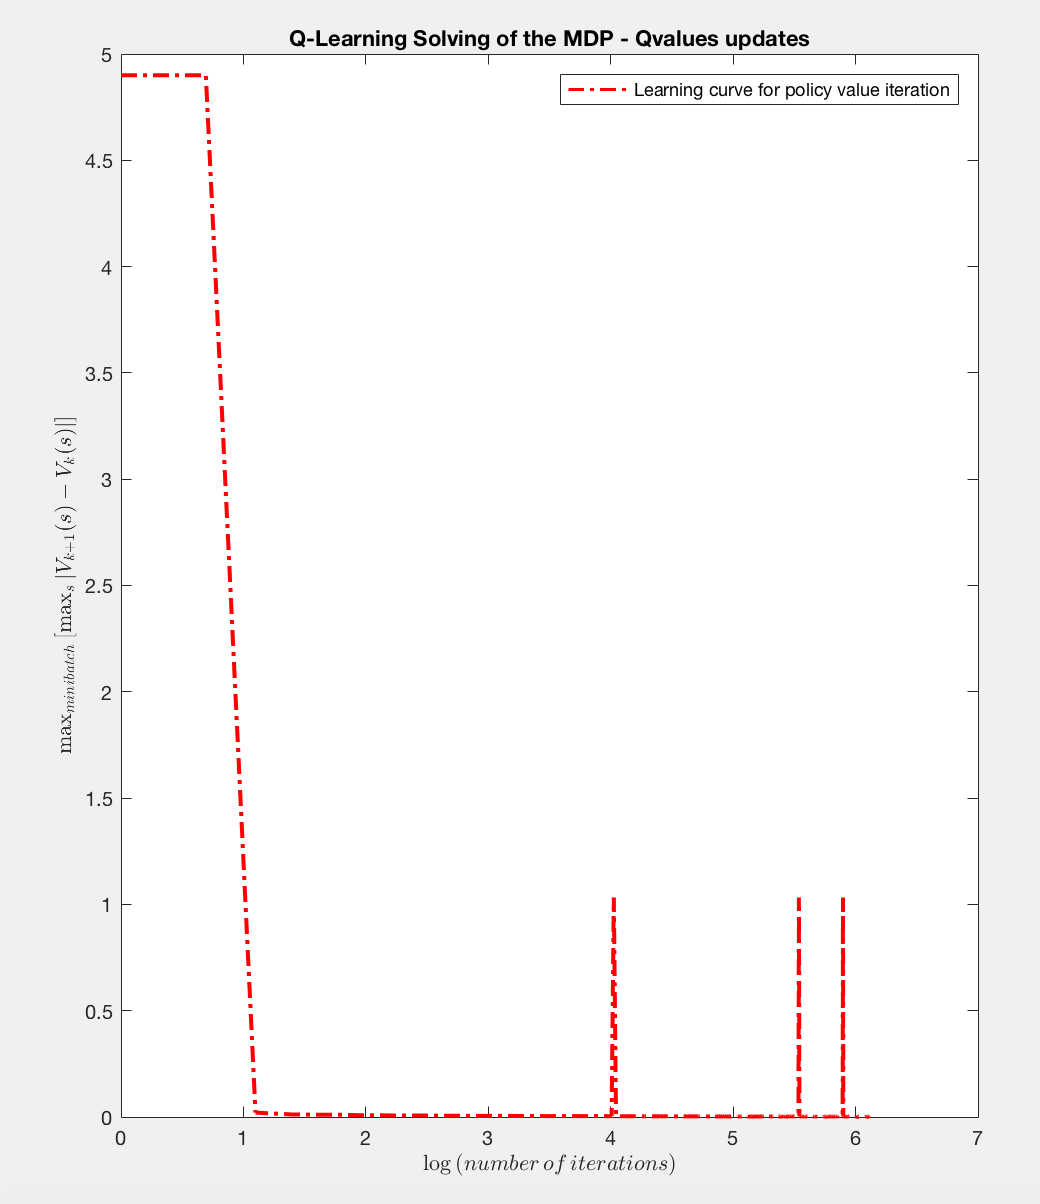
\includegraphics[width=\linewidth]{bargrid_ql_learning_curve}
						\caption{Learning curve for Q-learning on \emph{bar\_grid}}
					\end{minipage}
					\hfill
					\begin{minipage}{0.4\linewidth}
						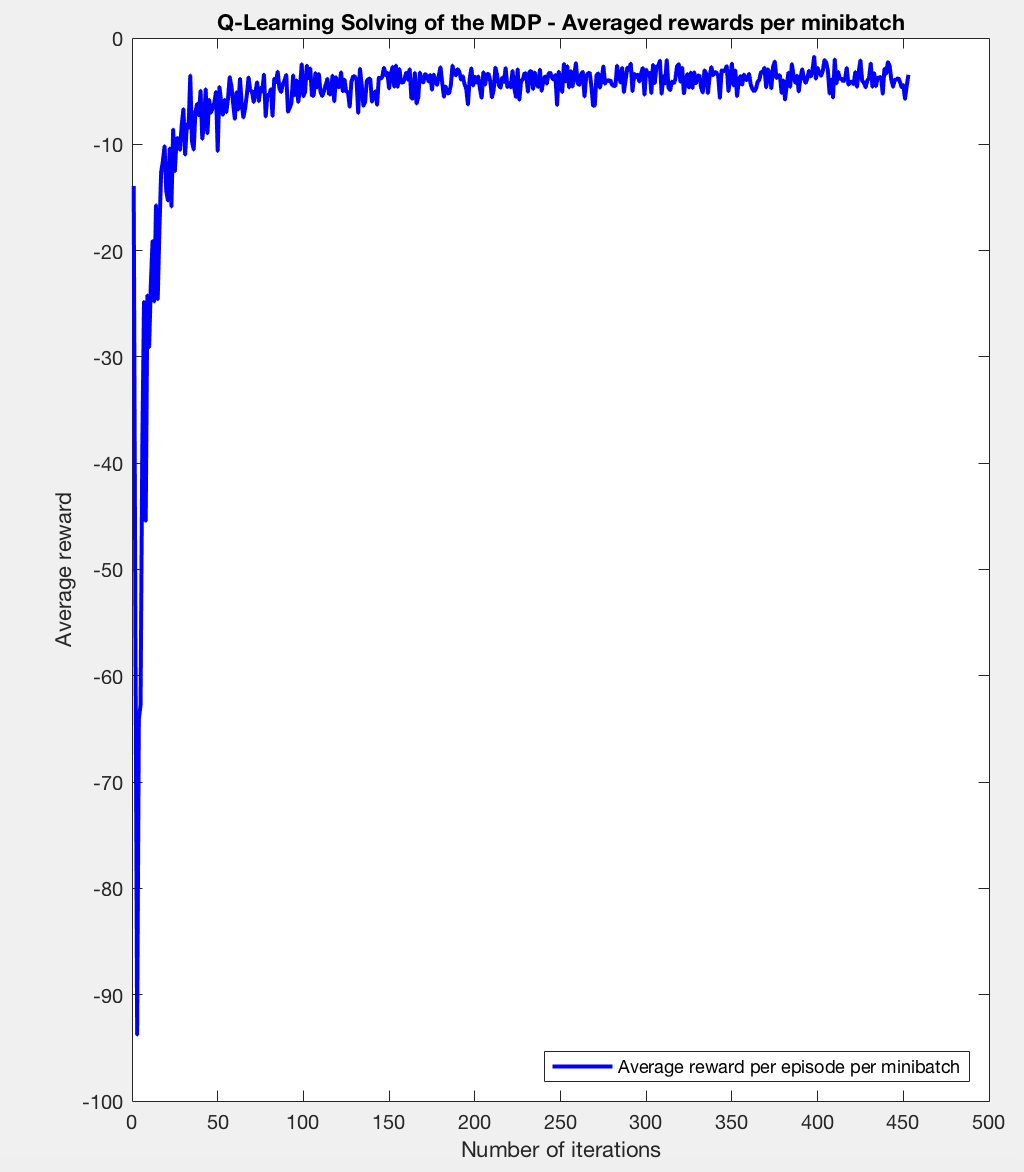
\includegraphics[width=\linewidth]{bargrid_ql_averaged_rewards}
						\caption{Averaged rewards over mini-batch for Q-learning on \emph{bar\_grid}}
					\end{minipage}
				\end{figure}

			}
		}
	}
	
	\chapter{Compliant-based reinforcement learning}
	{
		\section{Problem selection}
		{
			\paragraph{} With our approach, we wish to tackle two topics : on one hand, we wish to display a imitation based learning framework that \emph{accelerate} the learning process. Also, we wish to have a shifting compliance behavior so that an agent can \emph{overtake a suboptimal teacher}. We therefore needed to come up with a model that both learns slowly (with the algorithms discussed hereinbefore) and can get stuck in local minima. 
			
			\paragraph{} We chose the state space displayed in figure (\ref{fig::maze_display}). Every trajectory of the agent starts in the state colored with green. The agent first learn to reach for the first reward, but has to perform many exploratory moves in order to find the other reward, much bigger, and which systematic completion gives the optimal policy. Such a policy, first computed with dynamic programing, is displayed in figure (\ref{fig::maze_optimal_policy}). 
			
			\paragraph{} As displayed in figures (\ref{fig::maze_ql_lc}), (\ref{fig::maze_ql_ar}), (\ref{fig::maze_sarsa_lc}) and (\ref{fig::maze_sarsa_ar}), both algorithm with their fixed hyper-parameters learn slowly and can temporarily be stuck in local optima. This given problem therefore fits our expectations, and will now become our \textbf{baseline problem} for testing our different approaches. 
			
			\begin{figure}[h!]
				\begin{minipage}{0.45\linewidth}
					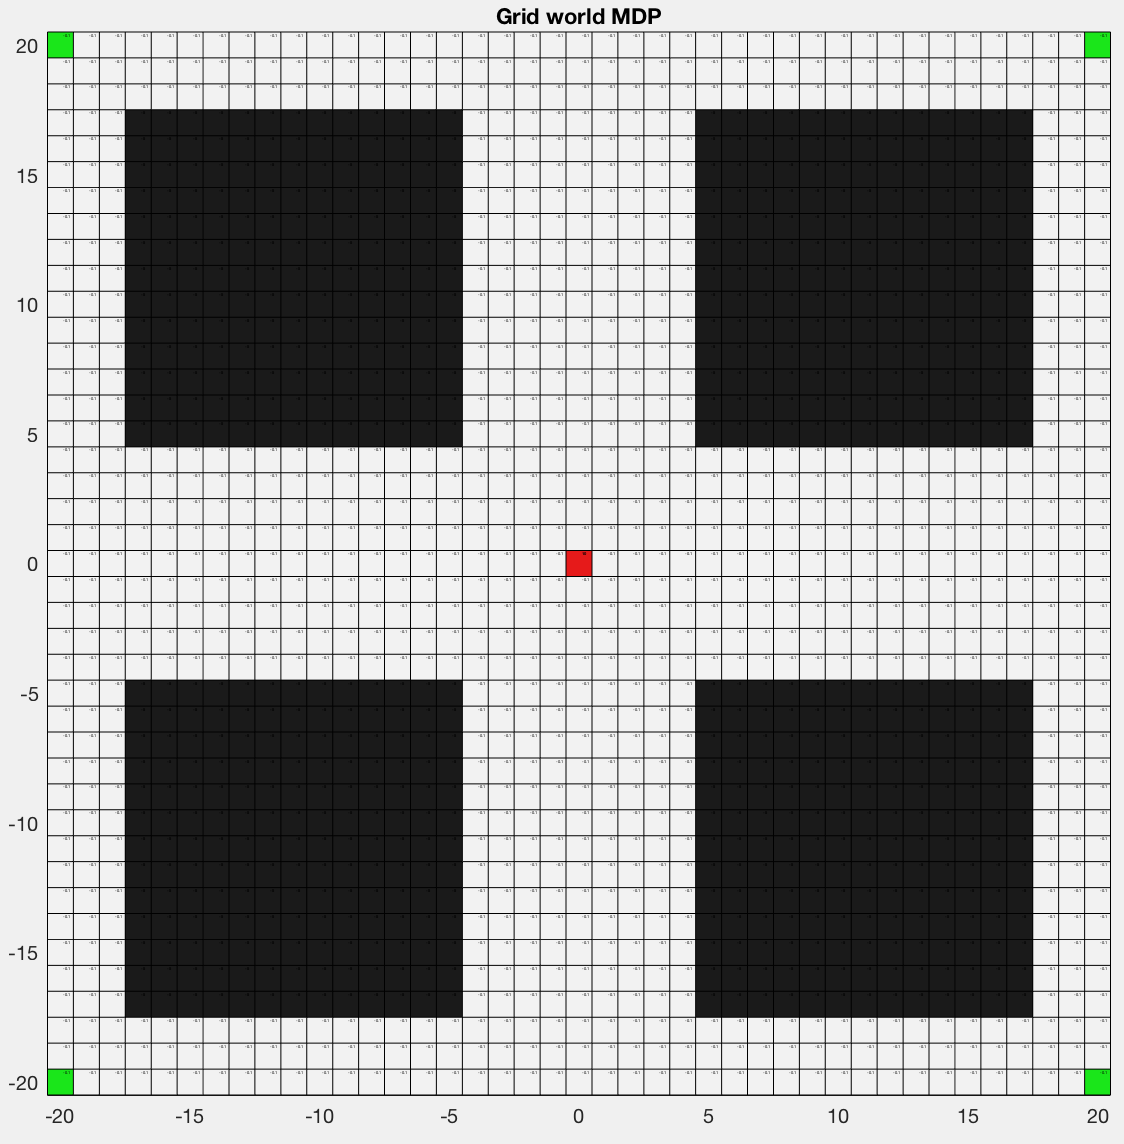
\includegraphics[width=\linewidth]{maze_grid}
					\caption{The \emph{maze\_grid} state space}
					\label{fig::maze_display}
				\end{minipage}
				\hfill
				\begin{minipage}{0.45\linewidth}
					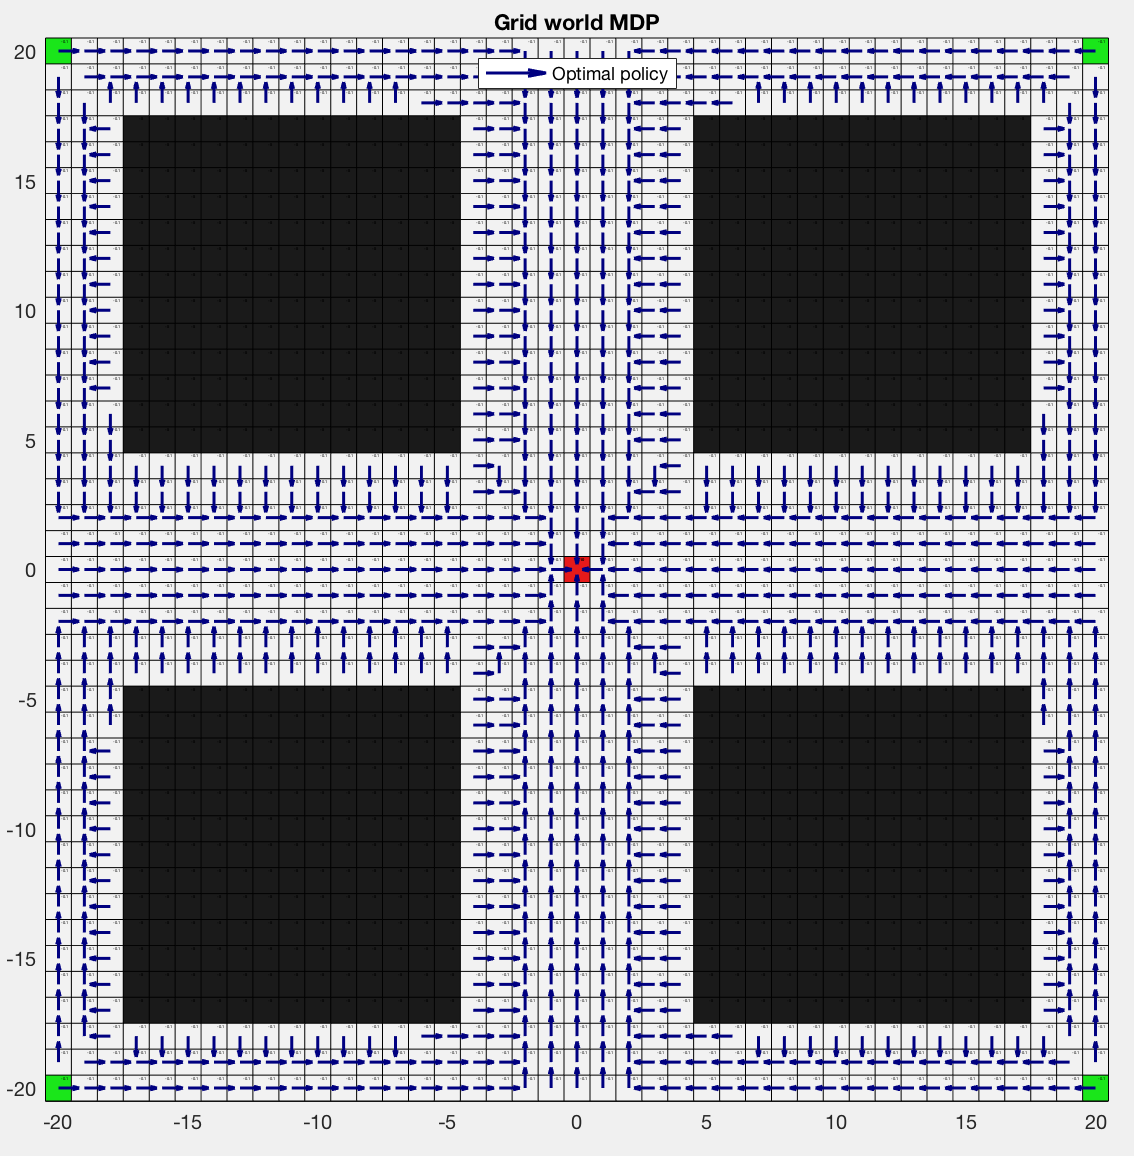
\includegraphics[width=\linewidth]{maze_optimal_policy}
					\caption{Optimal policy for the \emph{maze\_grid}, computed with DP}
					\label{fig::maze_optimal_policy}
				\end{minipage}
			\end{figure}
				
				
			\begin{figure}[h!]
				\begin{minipage}{0.45\linewidth}
					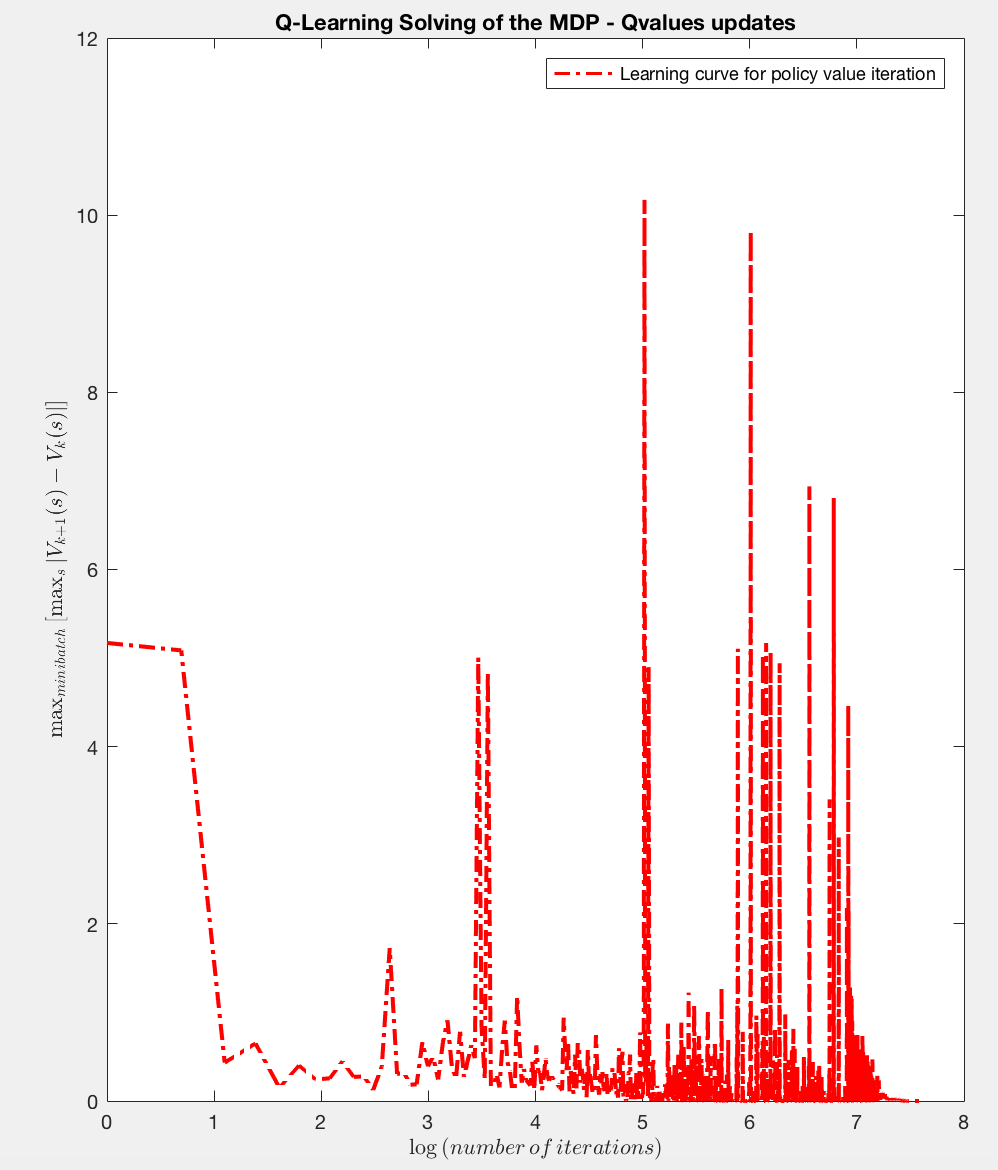
\includegraphics[width=\linewidth]{ql_maze_learning_curve}
					\caption{Learning curve for Q-learning on \emph{maze\_grid}}
					\label{fig::maze_ql_lc}
				\end{minipage}
				\hfill
				\begin{minipage}{0.45\linewidth}
					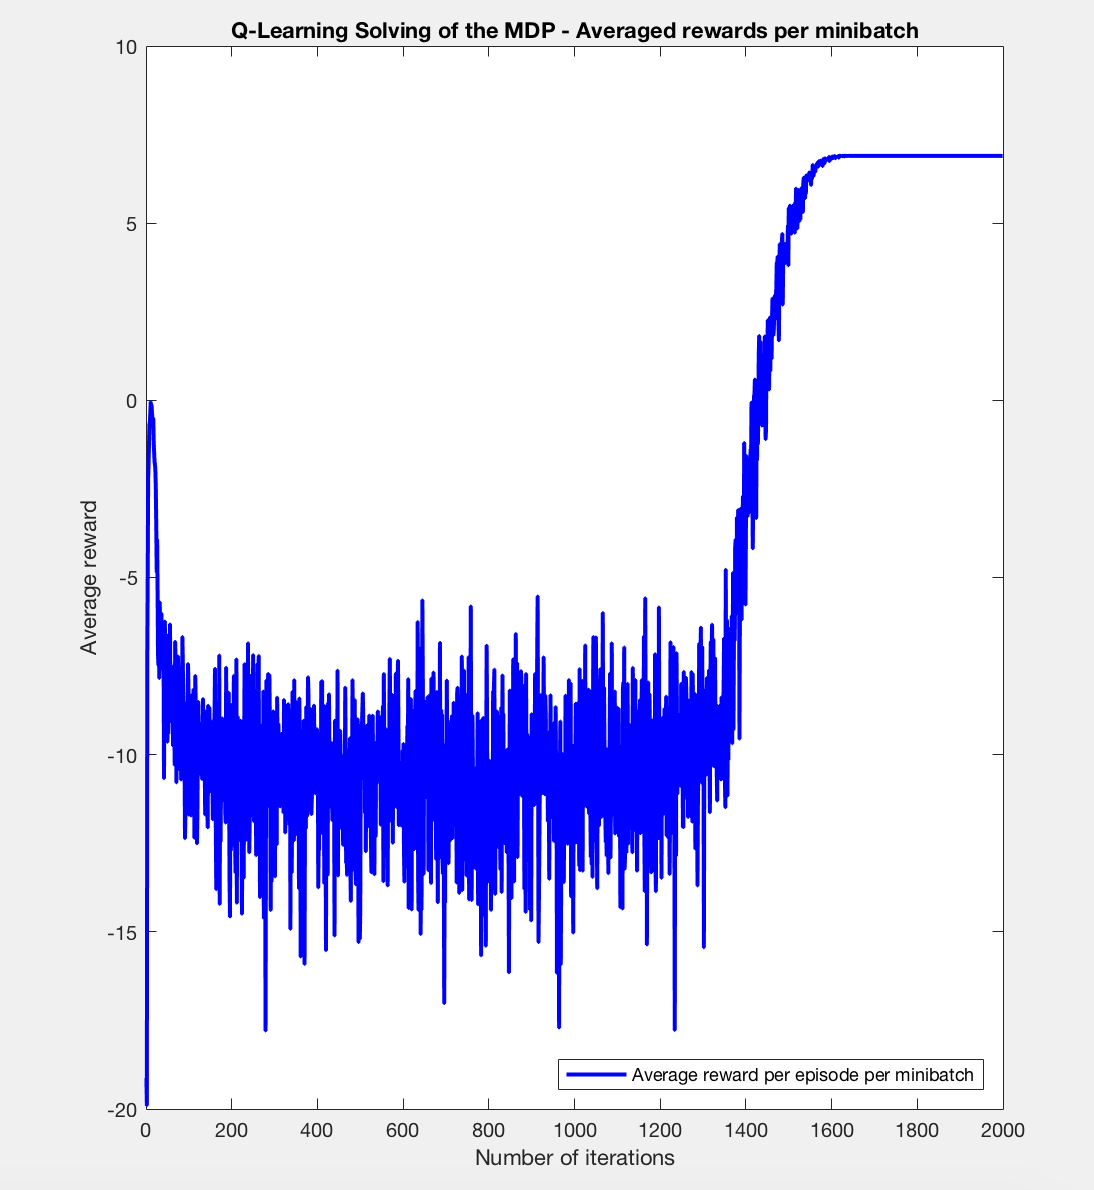
\includegraphics[width=\linewidth]{qlearn_maze_averaged_return}
					\caption{Averaged rewards over mini-batch for Q-learning on \emph{maze\_grid}}
					\label{fig::maze_ql_ar}
				\end{minipage}
			\end{figure}
			
			
			\begin{figure}[h!]
				\begin{minipage}{0.45\linewidth}
					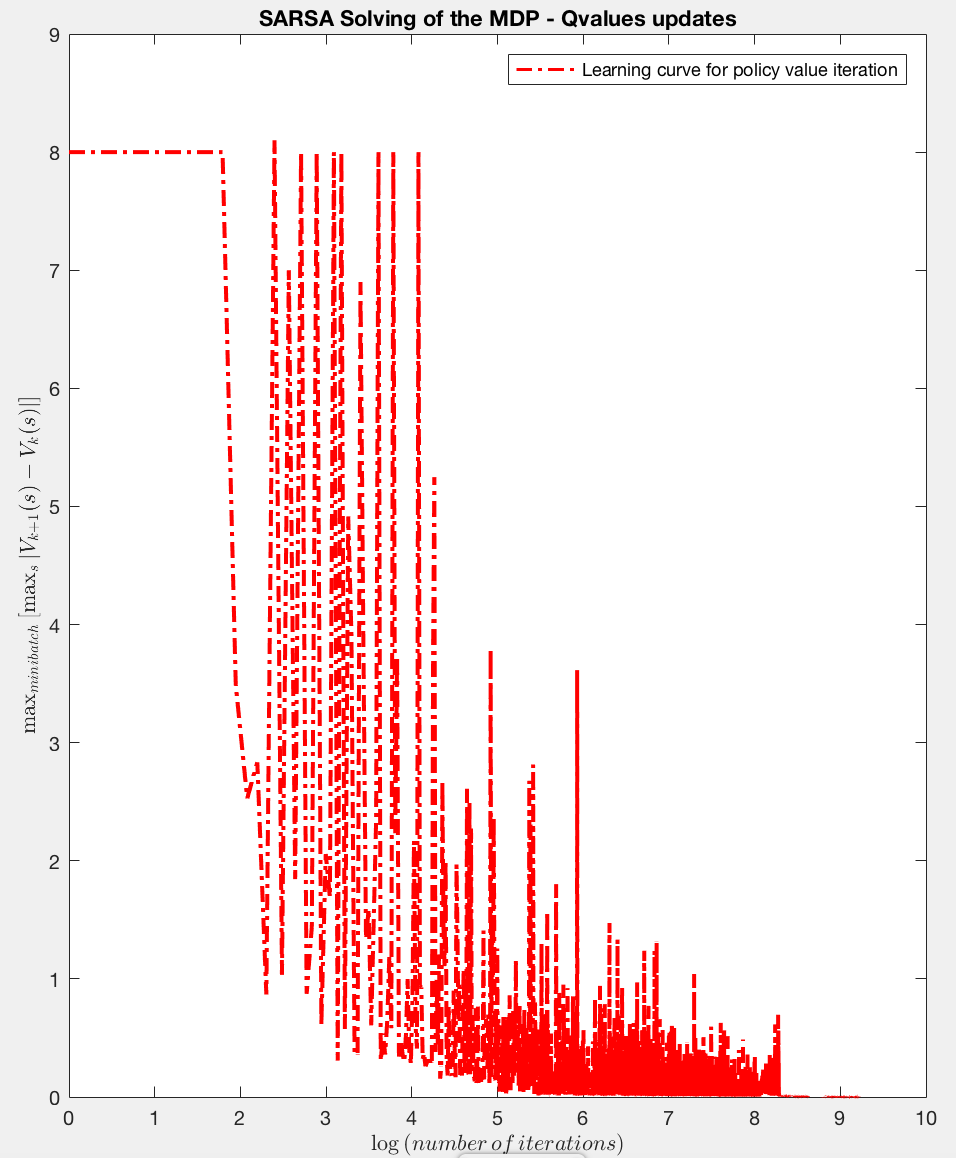
\includegraphics[width=\linewidth]{sarsa_maze_learning_curve}
					\caption{Learning curve for SARSA on \emph{maze\_grid}}
					\label{fig::maze_sarsa_lc}
				\end{minipage}
				\hfill
				\begin{minipage}{0.45\linewidth}
					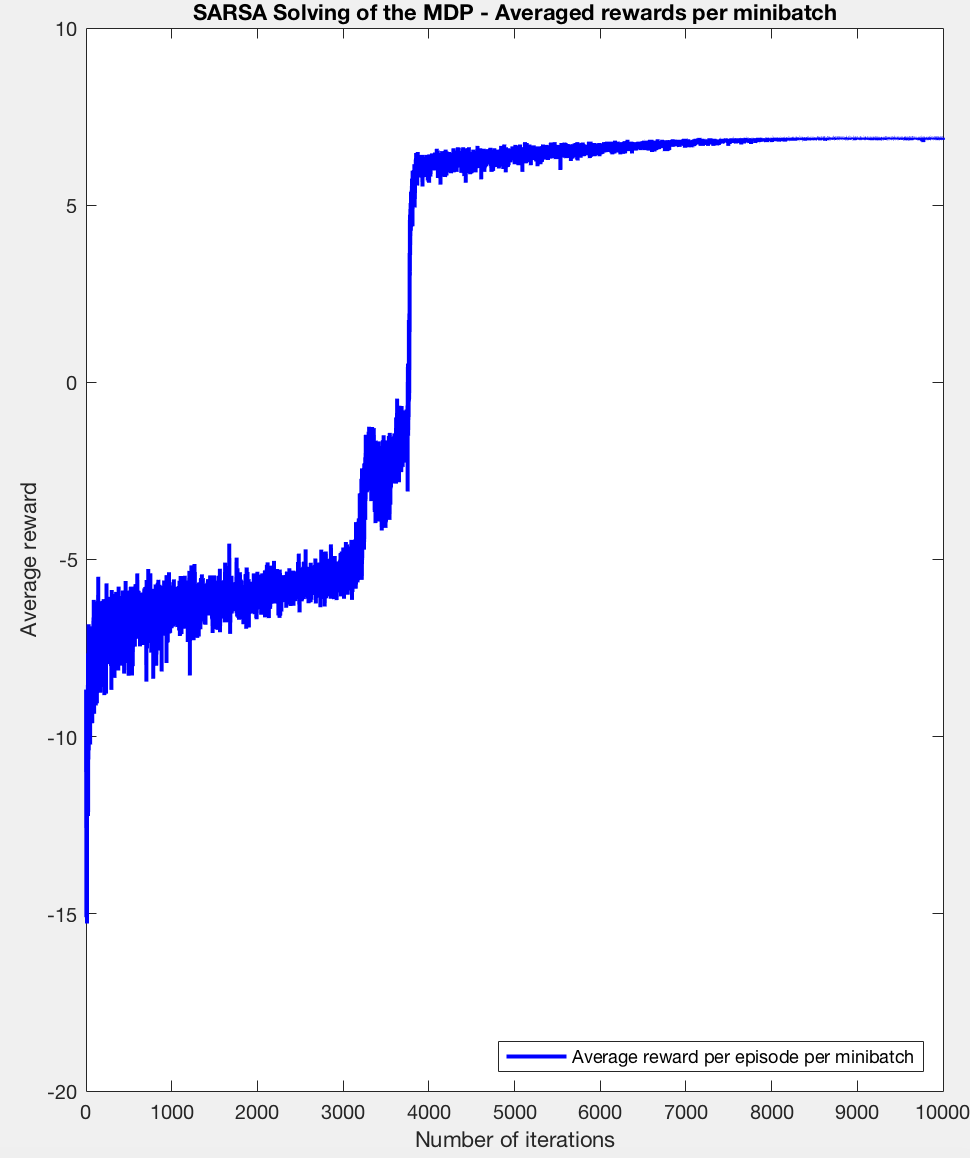
\includegraphics[width=\linewidth]{sarsa_maze_averaged_return}
					\caption{Averaged rewards over mini-batch for SARSA on \emph{maze\_grid}}
					\label{fig::maze_sarsa_ar}
				\end{minipage}
			\end{figure}
			
			
				
			
			\paragraph{} It is important to say that of course, hyper-parameters (initial temperature, optimistic initial Q-values, ..) for both problems can be tuned to accelerate learning. However, our point is here to address the fixed sub-optimal problem in order to prove our approach interest. 
		}
	}
	
	\chapter{Results}
	{
	
	}
	
	\chapter*{Conclusion}
	\addcontentsline{toc}{chapter}{Conclusion}
	
	
	\bibliographystyle{alpha}
 	 \bibliography{bibfile}
	 \nocite{*}
  
\end{document}